\documentclass[conference]{IEEEtran}
\usepackage{cite}
\usepackage{amsmath,amssymb,amsfonts}
\usepackage{algorithmic}
\usepackage{graphicx}
\usepackage{textcomp}
\usepackage{xcolor}
\usepackage{fancyhdr}
\usepackage[hyphens]{url}
\usepackage{tikz}

\def\BibTeX{{\rm B\kern-.05em{\sc i\kern-.025em b}\kern-.08em
    T\kern-.1667em\lower.7ex\hbox{E}\kern-.125emX}}

% Ensure letter paper
\pdfpagewidth=8.5in
\pdfpageheight=11in


%%%%%%%%%%%---SETME-----%%%%%%%%%%%%%
\newcommand{\iscasubmissionnumber}{NaN}
%%%%%%%%%%%%%%%%%%%%%%%%%%%%%%%%%%%%

\fancypagestyle{firstpage}{
  \fancyhf{}
\renewcommand{\headrulewidth}{0pt}
  \fancyhead[C]{\normalsize{ISCA 2021 Submission
      \textbf{\#\iscasubmissionnumber} \\ Confidential Draft: DO NOT DISTRIBUTE}}
  \fancyfoot[C]{\thepage}
}


\pagenumbering{arabic}

%%%%%%%%%%%---SETME-----%%%%%%%%%%%%%
\title{Distributed Near-Data Evaluating Complex Pooling Operations for Recommendation System's Embedding Tables}
\author{}
%%%%%%%%%%%%%%%%%%%%%%%%%%%%%%%%%%%%

\begin{document}
\maketitle
\thispagestyle{firstpage}
\pagestyle{plain}



%%%%%% -- PAPER CONTENT STARTS-- %%%%%%%%

\begin{abstract}

Recommendation system analyze long-term user behavior by 
first 1) extracting long user behavior sequences from huge embedding tables
distributed across servers connected by low bandwidth networks,
and then 2) reducing this long sequence with some pooling operators,
such as sum, soft searching and attention,
and finally 3) feeding the result into MLP.
Thus,
step 1 is the major performance bottleneck that accounts for over 80\% run time.

Recent studies have proposed near data processing (NDP) 
%and processing-in-memory (PIM)  
solutions for step 2, 
to reduce the long sequences before sending them across the low bandwidth network to GPUs.
But they can only handle simple sum pooling operators,
not the more complex soft searching and attention operator.

Thus,
this paper propose novel reformulations of soft searching 
and attention pooling operator with linear complexity,
and further propose new NDP architecture and communication protocol 
to evaluate them distributed on multiple DIMMs.

We implement this proposal in both FPGA and software prototype,
to respectively show it functional feasibility and performance advantage.
With xxx and xxx  benchmark,
we boost performance by xxx to xxx times.
We also analysis and show the area, power and merchant impact to the DIMM and whole system.
\end{abstract}

\section{Introduction}

Recommendation systems are widely used in
industry (e.g., 
Facebook \cite{recsys_dlrm_facebook}, 
Netflix\cite{recsys_netflix}, 
Youtube\cite{recsys_youtube}, 
Spotify\cite{recsys_spotify}, 
Baidu\cite{recsys_mobius_baidu},
Alibaba\cite{recsys_sim_alibaba}) 
to suggest content such as music, products, and videos to users. 
It directly drive revenues for these hyperscalers,
and therefore consume the vast majority,
over 80\% of AI inference \cite{ recsys_archimp_facebook_hpca20 } and more than 50\% of AI training \cite{ recsys_trainfb_facebook } ,
cycles in facebook.
Its annual growth rate are 3.3x for training \cite{recsys_trainfb_facebook} and 2X for inference \cite{recsys_inffb_facebook}.

As shown in Figure \ref{recsysLong}a),
a typical recommendation system training/inference flow contains the following components and steps:
\begin{enumerate}
\item A training sequence containing recent transactions,
for example,
web pages browsed by users,
items purchased by customers.
For each transaction,
the recommendation system not only extract the user id and item id accessed by this particular user, 
it also find out the sequence of items recently accessed by this user to capture the changing trend of this user profile.
This sequence is also called sparse feature as they are normally in one-hot format;
\item An embedding layer contains 10s to 100s of embedding tables,
each of which stores a set of real number feature vectors representing, 
for example,
an user, a web page or a song's profile.
For large E-commerce company like Alibaba,
the number of users and items often reach billions\cite{recsys_billionscale_alibaba},
which makes the embedding tables as large as 10TB and must be stored on multiple servers.
The sequence from step 1 will be used to index these embedding tables to find out their respective feature vectors;
\item A bottom MLP to map dense feature, 
such as age and time,
into feature vectors;
\item A top MLP to exploit the relation between all the feature vectors from above steps;
\end{enumerate}

\begin{figure}[tb]
\centering
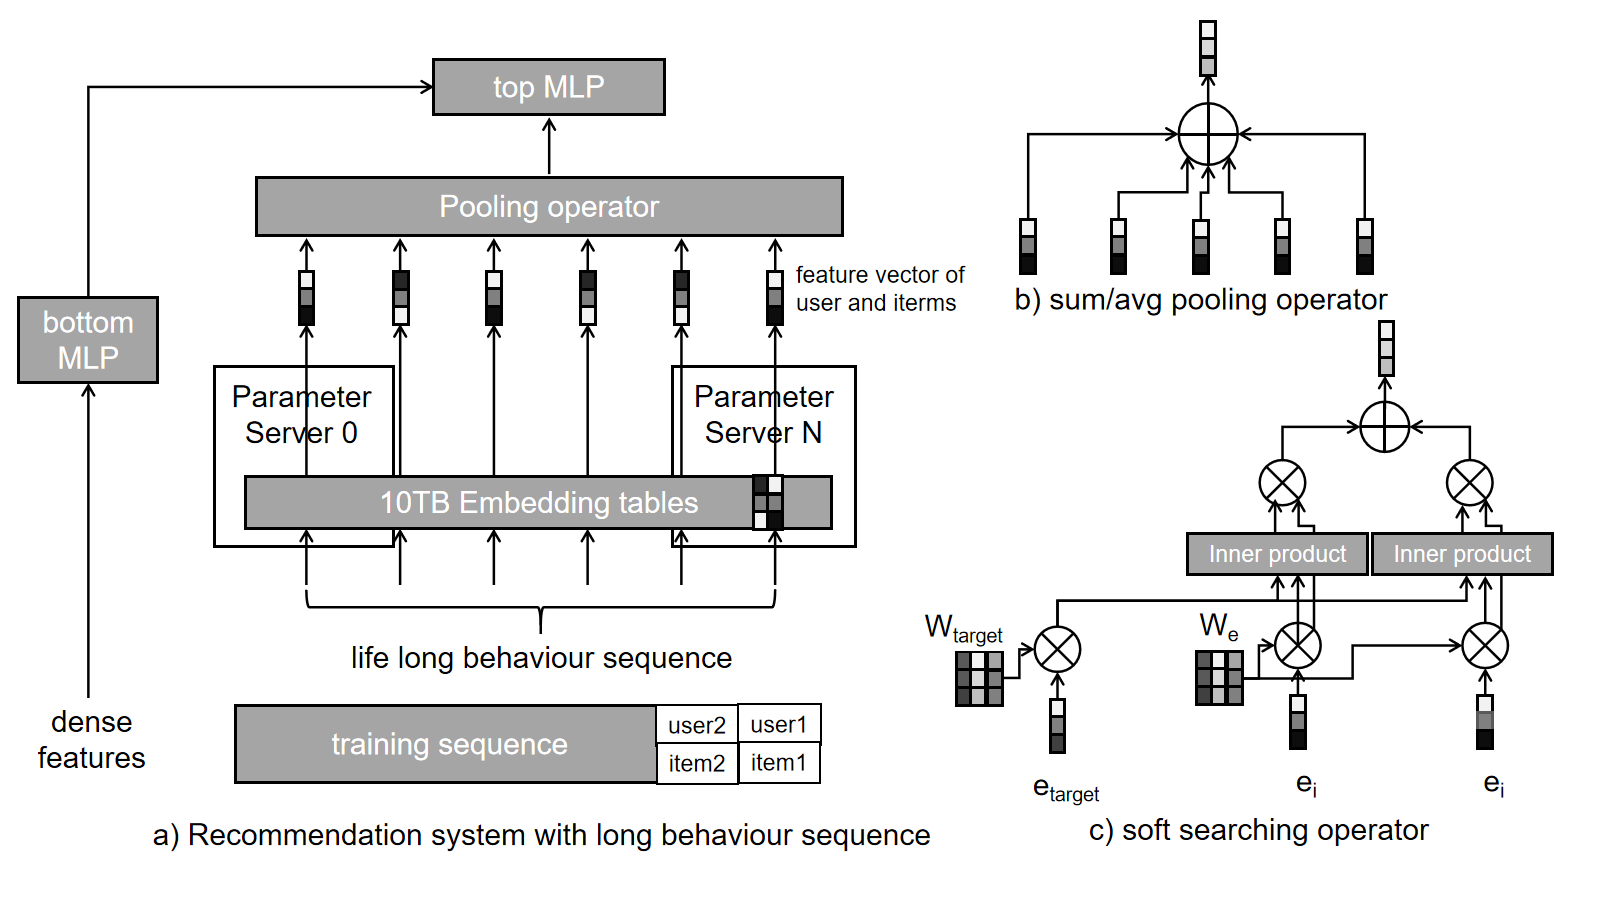
\includegraphics[width=0.5\textwidth]  {recsysLong.png}
\caption{Recommendation system with long user behavior sequences}
\label{recsysLong}
\end{figure}

Recent recommendation systems,
such as MIMN\cite{recsys_mimn_alibaba} and SIM\cite{recsys_sim_alibaba},
try to gain more in-depth insight into users long-term, 
even life long, behavior sequences,
whose length reach up to 54k in SIM\cite{recsys_sim_alibaba}.

However,
in spit of their significant accuracy improvement \cite{recsys_sim_alibaba},
it is a very time consuming task to load these long sequences across the low bandwidth network connecting
the servers storing huge 10TB embedding tables\cite{ recsys_baidu_aibox },
which account for more than 80\% of inference
\cite{recsys_archimp_facebook_hpca20 ,recsys_deeprecsys_facebook_isca20 } 
and training \cite{recsys_traineff_facebook_hpca21 } time.
Such overhead prevent these long sequence analysis from being deployed in production environment\cite{recsys_sim_alibaba},.

Recent proposals try to avoid this overhead by offloading the sum pooling operator into near-data processing (NDP) devices,
such as memory\cite{recacc_tensordimm_kaist_micro19 ,recacc_recnmp_facebook_isca20 , recacc_tensorcasting_kaist_hpca21 }, 
SSD \cite{recacc_recssd_kaist_asplos21 } and  network switch\cite{ recacc_fafnir_hpca21 }.
As shown in Figure \ref{recsysLong}b),
this sum pooling only need to sum up all these feature vectors coming out of the embedding tables,
which significantly reduce the size of feature vectors with little computation requirement.

However,
such proposals can not handle more complex pooling operators, 
such as soft searching in SIM \cite{recsys_sim_alibaba}
and attention in BST\cite{recsys_bst_alibaba},
which, as shown in Figure \ref{recsysLong}c),
contain matrix-vector multiplication operation posing 
heavy computation burden on the memory controller, SSD controller and network switch with 
very weak computation capability.

In this paper we new ideas to resolve these problem
such that complex soft searching and attention pooling operators can also be offloaded to NDP devices:
\begin{enumerate}
\item We propose  a new formulation of soft search and attention operators' forward and backward propagation algorithm,
such that the majority of matrix computation can be extracted out of inner loop,
and uploaded back to GPU.
Therefore,
only light weight vector-vector dot product need to be offloaded to NDP device,
while still significantly reduce the feature vectors.
\item We propose new communication protocols to collect necessary informance back to GPU to perform the matrix computation mentioned in step 1,
and to distribute the resulting vector back to NDP device to enable offloading.
\item We develop a noval NDP device architecture and implementation to implemente above computation.
\item We evalute the perfomance and compare it to state-of-the-art GPU and CPU implementation, and shown xxX and xxX performance advantage respectively.
\item We evalute its power and chip area efficiency.
\end{enumerate}




\section{Background}
\subsection{Recommendation System}


\subsection{}


\section{Reformulation of Complex Pooling Operators}
\subsection{Soft Searching}
Forward and Backward propagation

\subsection{Attention}


\section{System Design}
\subsection{System Architecture}
\subsection{Communication Protocol}
\subsection{Operator Mapping}



\section{Evaluation}
\subsection{Experimental Setup}
\subsection{Performance}

\subsection{Power}
We use CACTI \cite{cacti6} to evalute the power of this chip,
just like outerspace.

\subsection{Area}



\section{Related Work}

\section{Discussion}


\section{Conclusion}

\subsection{Format Highlights}

Here are the format highlights in a nutshell:
\begin{itemize}
\item Paper must be submitted in printable PDF format.
\item Text must be in a minimum 10pt Times font, see Table~\ref{table:formatting}.
\item Papers must be at most 11 pages (not including references) in a
  two-column format.
\item No page limit for references.
\item Each reference must specify {\em all} authors, i.e., no {\em et al.}
\end{itemize}

\subsection{Paper Evaluation Objectives}
The committee will make every effort to judge each submitted paper on
its own merits. There will be no target acceptance rate. We expect to
accept a wide range of papers with appropriate expectations for
evaluation --- while papers that build on significant past work with
strong evaluations are valuable, papers that open new areas with less
rigorous evaluation are equally welcome and especially encouraged. We
also acknowledge the wide range of evaluation methodologies in ISCA including
modeling, simulation, prototyping, experimental implementation, real
product evaluation, etc.
\subsection{Paper Formatting}
Papers must be submitted in printable PDF format and should contain a
{\em maximum of 11 pages} of single-spaced two-column text, {\bf not
  including references}.  You may include any number of pages for
references, but see below for more instructions.  If you are using
\LaTeX~\cite{lamport94} to typeset your paper, then we suggest that
you use the template used to prepare this document, which you can find
on the ISCA 2021 website. If you use a different
software package to typeset your paper, then please adhere to the
guidelines given in Table~\ref{table:formatting}.

\begin{scriptsize}
\begin{table}[h!]
  \centering
  \caption{Formatting guidelines for submission.}
  \label{table:formatting}
  \begin{tabular}{|l|l|}
    \hline
    \textbf{Field} & \textbf{Value}\\
    \hline
    \hline
    File format & PDF \\
    \hline
    Page limit & 11 pages, {\bf not including}\\
               & {\bf references}\\
    \hline
    Paper size & US Letter 8.5in $\times$ 11in\\
    \hline
    Top margin & 1in\\
    \hline
    Bottom margin & 1in\\
    \hline
    Left margin & 0.75in\\
    \hline
    Right margin & 0.75in\\
    \hline
    Body & 2-column, single-spaced\\
    \hline
    Space between columns & 0.25in\\
    \hline
    Line spacing (leading) & 11pt \\
    \hline
    Body font & 10pt, Times\\
    \hline
    Abstract font & 10pt, Times\\
    \hline
    Section heading font & 12pt, bold\\
    \hline
    Subsection heading font & 10pt, bold\\
    \hline
    Caption font & 9pt (minimum), bold\\
    \hline
    References & 8pt, no page limit, list \\
               & all authors' names\\
    \hline
  \end{tabular}
\end{table}
\end{scriptsize}

{\em Please ensure that you include page numbers with your
  submission}. This makes it easier for the reviewers to refer to
different parts of your paper when they provide comments. Please
ensure that your submission has a banner at the top of the title page,
similar to this document, which contains the submission number and the
notice of confidentiality.  If using the template, just replace `NaN'
with your submission number.

\subsection{Content}
Reviewing will be {\em double blind} (no author list); therefore,
please do not include any author names on any submitted documents
except in the space provided on the submission form.  You must also
ensure that the metadata included in the PDF does not give away the
authors. If you are improving upon your prior work, refer to your
prior work in the third person and include a full citation for the
work in the bibliography.  For example, if you are building on {\em
  your own} prior work in the
papers~\cite{nicepaper1,nicepaper2,nicepaper3}, you would say
something like: "While the authors of~\cite{nicepaper1,nicepaper2,nicepaper3} did X,
Y, and Z, this paper additionally does W, and is therefore much
better."  Do NOT omit or anonymize references for blind review.  There
is one exception to this for your own prior work that appeared in IEEE
CAL, arXiv, workshops without archived proceedings, etc.\ as
discussed later in this document.

\noindent\textbf{Figures and Tables:} Ensure that the figures and
tables are legible.  Please also ensure that you refer to your figures
in the main text.  Many reviewers print the papers in
gray-scale. Therefore, if you use colors for your figures, ensure that
the different colors are highly distinguishable in gray-scale.

\noindent\textbf{References:}  There is no length limit for
references. {\em Each reference must explicitly list all authors of
  the paper.  Papers not meeting this requirement will be rejected.}
Since there is no length limit for the number of pages
used for references, there is no need to save space here.


\section{Paper Submission Instructions}

\subsection{Guidelines for Determining Authorship}
IEEE guidelines dictate that authorship should be based on a {\em
  substantial intellectual contribution}. It is assumed that all
authors have had a significant role in the creation of an article that
bears their names. In particular, the authorship credit must be
reserved only for individuals who have met each of the following
conditions:

\begin{enumerate}
\item Made a significant intellectual contribution to the theoretical
  development, system or experimental design, prototype development,
  and/or the analysis and interpretation of data associated with the
  work contained in the article;

\item Contributed to drafting the article or reviewing and/or revising
  it for intellectual content; and

\item Approved the final version of the article as accepted for publication, including references.
\end{enumerate}

A detailed description of the IEEE authorship guidelines and
responsibilities is available online.\footnote{\url{https://www.ieee.org/publications_standards/publications/rights/Section821.html}} Per
these guidelines, it is not acceptable to award {\em honorary}
authorship or {\em gift} authorship. Please keep these guidelines in
mind while determining the author list of your paper.

\subsection{Declaring Authors}
Declare all the authors of the paper upfront. Addition/removal of
authors once the paper is accepted will have to be approved by the
program chair, since it potentially undermines the goal of eliminating
conflicts for reviewer assignment.

\subsection{Areas and Topics}
Authors should indicate specific topics covered by the paper on the
submission page. If you are unsure whether your paper falls within the
scope of ISCA, please check with the program chair --- ISCA is a broad,
multidisciplinary conference and encourages new topics.

\subsection{Declaring Conflicts of Interest}

Authors must register all their conflicts on the paper submission
site. Conflicts are needed to ensure appropriate assignment of
reviewers. If a paper is found to have an undeclared conflict that
causes a problem OR if a paper is found to declare false conflicts in
order to abuse or `game' the review system, the paper may be rejected.

Please declare a conflict of interest with the following people for any author of your paper.
A conflict occurs in the following cases:
\begin{enumerate}
\item Between advisor and advisee forever.
\item Between family members forever.
\item Between people who have collaborated in the last 5 years. This
  collaboration can consist of a joint research or development
  project, a joint paper, or when there is direct funding from the
  potential reviewer (as opposed to company funding) to an author of
  the paper. Co-participation in professional activities, such as
  tutorials or studies, is not cause for conflict. When in doubt, the
  author should check with the Program Chair.
\item Between people from same institution or who were in the same
  institution in the last 5 years.
\item Between people whose relationship prevents the reviewer from
  being objective in his/her assessment.
\end{enumerate}

`Service' collaborations, such as co-authoring a report for a
professional organization, serving on a program committee, or
co-presenting tutorials, do not themselves create a conflict of
interest. Co-authoring a paper that is a compendium of various
projects with no true collaboration among the projects does not
constitute a conflict among the authors of the different projects. On
the other hand, there may be others not covered by the above with whom
you believe a COI exists, for example, an ongoing collaboration which
has not yet resulted in the creation of a paper or proposal. Please
report such COIs; however, you may be asked to justify them. Please be
reasonable. For example, you cannot declare a COI with a reviewer just
because that reviewer works on topics similar to or related to those
in your paper.  The program chair may contact co-authors to explain a COI
whose origin is unclear.

Most reviews will be solicited among the members of the PC and the ERC, but other
members from the community may also write reviews. Please declare all
your conflicts (not just restricted to the PC and ERC) on the
submission form. When in doubt, contact the program chair.


\subsection{Concurrent Submissions and Workshops}
By submitting a manuscript to ISCA 2021, the authors guarantee that
the manuscript has not been previously published or accepted for
publication in a substantially similar form in any conference,
journal, or the archived proceedings of a workshop (e.g., in the
ACM/IEEE digital libraries) --- see exceptions below. The authors also
guarantee that no paper that contains significant overlap with the
contributions of the submitted paper will be under review for any
other conference or journal or an archived proceedings of a workshop
during the ISCA 2021 review period. Violation of any of these
conditions will lead to rejection.

The only exceptions to the above rules are for the authors' own papers
in (1) workshops without archived proceedings such as in the ACM/IEEE
digital libraries (or where the authors chose not to have their paper
appear in the archived proceedings), or (2) venues such as IEEE CAL or
arXiv where there is an explicit policy that such publication does not
preclude longer conference submissions.  In all such cases, the
submitted manuscript may ignore the above work to preserve author
anonymity. This information must, however, be provided on the
submission form --- the program chair will make this information available
to reviewers if it becomes necessary to ensure a fair review.
If you have already put your manuscript on arXiv, in the interest of
double blind review, modify the title for the version you submit to ISCA.
As always, if you are in doubt, it is best to contact program chairs.


Finally, the ACM/IEEE Plagiarism Policies\footnote{\url{http://www.acm.org/publications/policies/plagiarism_policy}\\
\url{https://www.ieee.org/publications_standards/publications/rights/plagiarism_FAQ.html}}
cover a range of ethical issues concerning the misrepresentation of
other works or one's own work.


\section*{Acknowledgements}
This document is derived from previous conferences, in particular ISCA
2019, MICRO 2019, ISCA 2020, and MICRO 2020.

%%%%%%% -- PAPER CONTENT ENDS -- %%%%%%%%


%%%%%%%%% -- BIB STYLE AND FILE -- %%%%%%%%
\bibliographystyle{IEEEtranS}
\bibliography{refs}
%%%%%%%%%%%%%%%%%%%%%%%%%%%%%%%%%%%%

\end{document}

